\documentclass[11pt,a4paper]{article}
\usepackage[hyperref]{acl2018}
\usepackage{times}
\usepackage{latexsym}
\usepackage{float}
\usepackage{graphicx}
\usepackage{url}
\usepackage{lingmacros}
\usepackage{arydshln}
\usepackage{gb4e}
\noautomath
\hypersetup{draft} % remove the draft later, issues caused by urls in footnote
\usepackage{enumitem}
% \setlist[description]{noitemsep}
\renewcommand{\arraystretch}{1.25}

\newcommand\BibTeX{B{\sc ib}\TeX}

\title{Economic Event Detection in Company-Specific News Text}

%\author{First Author \\
  %Affiliation / Address line 1 \\
  %Affiliation / Address line 2 \\
  %Affiliation / Address line 3 \\
  %{\tt email@domain} \\\And
  %Second Author \\
  %Affiliation / Address line 1 \\
  %Affiliation / Address line 2 \\
  %Affiliation / Address line 3 \\
 % {\tt email@domain} \\}

\date{}

\begin{document}
\maketitle
\begin{abstract}
This paper presents a dataset and supervised classification approach for economic event detection in English news articles.
Currently, the economic domain is lacking resources and methods for data-driven supervised event detection.
The task is conceived as a sentence-level classification task for 10 different economic event types.
Two different machine learning approaches were applied for the task: a rich feature set Support Vector Machine (SVM) set-up and a word-vector-based long short-term memory recurrent neural network (RNN-LSTM) set-up.
We show satisfactory results for most event types, with the linear kernel SVM outperforming the other experimental set-ups.
\end{abstract}
\section{Introduction}

In the financial domain, the way companies are perceived by investors is influenced by the news published about those companies \cite{Engle1993, Tetlock2007, Mian2012}.
\citet{Tetlock2007}, for example, tried to characterize the relationship between the content of media reports and daily stock market activity, focusing on the immediate influence of the Wall Street Journal's `Abreast of the Market' column on U.S. stock market returns.
One of his major findings was that high levels of media pessimism robustly predict downward pressure on market prices.

To provide some insights into the way markets react to new information about companies, financial economists have conducted “event studies”.
These event studies measure the impact of a specific event on the value of a firm~\cite{MacKinlay1997}. They
offer insight into the extent to which shareholders of acquired firms gain better returns during mergers, or examine the behavior of companies’ stock prices around events such as dividend announcements or stock splits. 
Studying the impact of specific events on the stock markets, however, is a labor-intensive process, starting with the identification of a given event, the estimation of abnormal returns to separate the general movement of stock returns from an individual stock return, followed by a number of statistical tests seeking evidence to support the event's economic significance.
Since identifying news published about certain events in an automatic way enables researchers in the field of event studies to process more data in less time, and can consequently lead to new insights into the correlation between events and stock market movements, automatic techniques have been proposed to detect economic events in text.

Most of the existing approaches to the detection of economic events, however, are knowledge-based and pattern-based \cite{Arendarenko2012, Hogenboom2013, du2016puls}.
These use rule-sets or ontology knowledge-bases which are largely or fully created by hand.
The Stock Sonar project~\cite{feldman2011stock} notably uses domain experts to formulate event rules for rule-based stock sentiment analysis.
This technology has been successfully used in assessing the impact of events on the stock market~\cite{boudoukh2016information} and in formulating trading strategies~\cite{ben2017event}.
Other approaches conceptualize economic event detection as the extraction of event tuples~\cite{Ding:2015:DLE:2832415.2832572} or as semantic frame parsing~\cite{xie2013semantic}.

A drawback of knowledge-based information extraction methods is that creating rules and ontologies is a difficult, time-consuming process.
Furthermore, defining a set of strict rules often results in low recall scores, since these rules usually cover only a portion of the many various ways in which certain information can be lexicalized.
Thus, the need for flexible data-driven approaches, which do not require predefined ontological resources, arises. We are not aware of any published data-driven, supervised event detection approaches for the economic domain. However, in general domain event extraction as embodied by projects such as ACE~\cite{ahn2006stages} and ERE/TAC-KBP~\cite{mitamura2016overview}, supervised methods for extraction of event structures are predominant because of their promise of improved performance.

As discussed in \citet{sprugnoli2017one}, the definition of events in the field of information extraction differs widely.
In this work, we employ a conceptualization of economic event detection as `retrieving textually reported real-world occurrences, actions, relations, and situations involving companies and firms'.
Unlike other supervised data-driven `event extraction' tasks such as in the ACE/ERE programs \cite{aguilar2014comparison}, we do not conceptualize events as structured schemata/frames, but more limited as textual mentions of real-world occurrences.
The task presented here is often also referred to as event `mention', `nugget', or `trigger' detection.
The classification experiments described here are currently at the sentence-level, but our event annotation scheme is token-level.

In this paper, we tackle the task of economic event detection by means of a supervised machine learning approach, which we expect will be able to detect a wider variety of lexicalizations of economic events than pattern-based approaches.
We consider economic event detection as a sentence-level multi-label classification task.
The goal is to automatically assign the presence of a set of pre-determined economic event categories in a sentence of a news article.

We compare two different machine learning approaches, viz.~a rich feature set Support Vector Machine (SVM) approach, and a word-vector-based sequence long short-term memory recurrent neural network (RNN-LSTM) approach.
We show that supervised classification is a viable approach to extract economic events, with the SVM linear kernel obtaining the best classification performance.

The remainder of this paper is structured as follows. In Section~\ref{datadescription}, we present the annotated corpus of financial news articles we constructed.
Section~\ref{experimentalsetup} introduces our two classification approaches to economic event detection, followed by an overview of the results in Section~\ref{resultsanddiscussion}. In Section~\ref{errorAnalysis}, we conduct an error analysis to gain insights in the main shortcomings of the current approach.  
Section~\ref{sec:conclusions} formulates some conclusions and ideas for future work.

\section{Data Description} \label{datadescription}

In this section, we describe the SentiFM economic event dataset collection and annotation.
The annotated dataset consists of an English and Dutch news corpus.
While in this paper the focus is on English, we refer to \citet{lefever2016dutcheventdetection} for a pilot study on Dutch event detection and a description of the Dutch event data.
A reference to where to download the SentiFM dataset can be found in Section~\ref{sec:dataavailability}.

The goal of the SentiFM dataset is to enable supervised data-driven event detection in company-specific economic news.
For English, we downloaded articles from the newspaper The Financial Times using the ProQuest Newsstand by means of keyword-search.
The keywords were manually determined based on a subsample of random articles as being indicative to one of the event types.
All articles were published between November 2004 and November 2013.
The articles had at least one of the following seven companies in the title: Barclays, BHP, Unilever, British Land, Tesco, Vodafone, and BASF.
These companies were selected because they are highly ranked in several market indexes while situated in different sectors/industries.
This facilitates corpus collection as there is more news content due to the companies' status.
Sectorial diversification is necessary to avoid specialization to one particular industry.
For instance, six out of 10 highest market cap companies in the S\&P500 index currently belong to the IT sector.
In total, we collected 497 news articles containing 2522 annotated company-specific economic events.

In the corpus, 10 types of company-specific economic events were manually identified:
\begin{description}
    \item [Buy ratings] A recommendation to purchase the security from an analyst. As event mentions, we include rating announcements, forecasts, performance, buy/sell/hold advice, and rating upgrades/downgrades/maintained.
    \item [Debt] Event mentions pertaining to company debt and debt ratios. We include debt announcements, forecasts, increases, reductions, and restructuring. 
    \item [Dividend] A dividend is a distribution of a portion of a company's earnings paid to its shareholders. We include dividend announcements, forecasts, payments, none payments, stable yields, raises, and reductions.
    \item [Merger \& acquisition] Mergers and acquisitions refers to the consolidation of companies or assets involving at least two companies. We include announcements, forecasts, and cancellations of a merger/acquisition.
    \item [Profit] Financial benefits that are realized when the amount of revenue exceeds expenses. We include declarations and forecasts of profit, positive and negative (losses) profit, lower than, higher than, as expected, increased, decreased, and stable profits.
    \item [Quarterly results] Events pertaining to the quarterly report as a set of financial statements issued by a company. We include declaration of publication, forecasts, strong, weak, improved, declined, stable, better than, worse than, and as expected results.
    \item [Sales volume] The quantity of goods and services sold over a certain period. We include declarations and predictions of sales volumes figures, increased, decreased, stable, better than, worse than, as expected sales volumes.
    \item [Share repurchase] Share buyback events by a company including announcements and forecasts of share repurchases.
    \item [Target price] Events on the projected price level of a security. We include announcements, forecasts, price raised, reduced, or maintained.
    \item [Turnover] The number and frequency of securities traded over a certain period. We include declaration and prediction of turnover figures, increased, decreased, stable, worse than, better than, and as expected turnover.
\end{description}

These events and activities pertain to the specific instances of companies mentioned in the articles.
The event typology was manually and iteratively constructed on a corpus subsample by an economic domain specialist.
It is notable that this event typology overlaps with the independently created StockSonar typology~\cite{feldman2011stock}.
Events are linked to the earliest preceding company mentions with an `about\_company' relation (this relation is duplexed into `acquiring\_company' and `target\_company' for Merger \& acquisition events).
Human annotators marked all mentions of each of these event types at the token level, using the Brat rapid annotation tool~\cite{Stenetorp2012}, a web-based tool for text annotation.
Discontinuous token spans and annotating multiple event types are allowed.

All texts were pre-processed (tokenized and sentence-splitted) using the LeTs Preprocess Toolkit~\cite{VandeKauter2013}.

\begin{table}[!htb]
	\centering
	\small{
		\begin{tabular}{l r r}
			\textbf{Event type} & \textbf{Type ratio} & \textbf{$\#$ sentence instances}   \\   
			\hline                                       
			No Event            & NA                  & 7823 (75.62\%)                     \\
			BuyRating           & 9.00\%              & 227 (2.19\%)                       \\
			Debt                & 2.38\%              & 60 (0.58\%)                        \\
			Dividend            & 7.22\%              & 182 (1.76\%)                       \\
			MergerAcquisition   & 10.03\%             & 253 (2.45\%)                       \\
			Profit              & 25.81\%             & 651 (6.29\%)                       \\
			QuarterlyResults    & 10.59\%             & 267 (2.58\%)                       \\
			SalesVolume         & 19.31\%             & 487 (4.71\%)                       \\
			ShareRepurchase     & 2.42\%              & 61 (0.59\%)                        \\
			TargetPrice         & 3.73\%              & 94 (0.91\%)                        \\
			Turnover            & 9.52\%              & 240 (2.32\%)                       \\
			\hdashline                                   
			Total               & \multicolumn{2}{r}{2522 events/10345 sentences (24.38\%)}\\
		\end{tabular}
		\caption{Event type distribution in the SentiFM English economic dataset and sentence level counts (as used in experiments).}
		\label{tab:instances}
	}
\end{table}

\begin{figure*}[!htb]
    \centering
    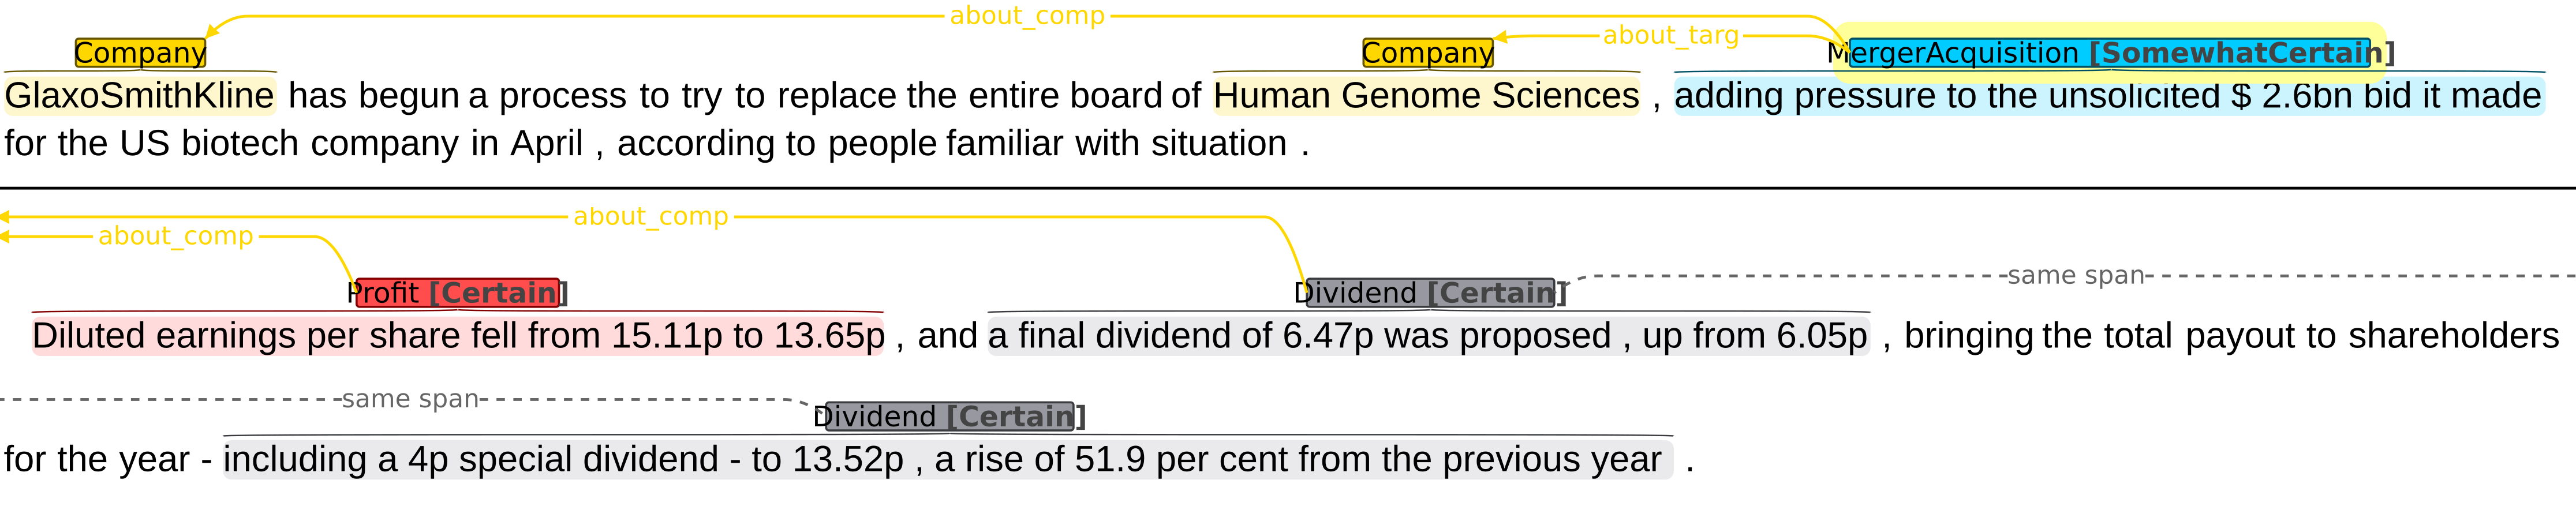
\includegraphics[width=\textwidth]{figures/annexamples600dpi.png}
    \caption{Annotated sentence examples from the Brat annotation tool.}
    \label{fig:bratexamples}
\end{figure*}

The present task is sentence-level detection of event types, so one sentence instance can be assigned multiple event classes.
Multiple labels are assigned to 3.81\% ($n=380$) of all sentence instances.
An overview of the different event types and their total frequency is given in Table~\ref{tab:instances}.

\section{Experimental Set-up} \label{experimentalsetup}

For this study, the task of economic event detection is conceived as a sentence-level classification task.
We decided on comparing two different machine learning approaches: an SVM approach requiring offline feature engineering, and a word-vector-based sequence RNN-LSTM approach.

The SVM approach incorporates a rich feature set with syntactic and lexical feature engineering.
We built one SVM classifier per event, predicting whether the event was present in the sentence or not, in effect recasting the problem as a one-vs-rest binary classification task for each class.
The RNN-LSTM is tested both as a multi-label single model classifier and a one-vs-rest set-up.

Performance estimation is done on a random hold-out test split (10\%), whereas cross-validation experiments were carried out on the hold-in set (train set of 90\%) for both hyper-parameter optimization and validation of generalization error.
%The performance metric used for picking the winning model in hyper-parameter search is $F_1$-score.
%For the SVM approach, the winning hyper-parametrization of a single binary classifier is determined by $F_1$-score computed over the positive class.

Per event type, precision, recall, and $F_1$-score are reported for each approach on the hold-out test set.
We do not report accuracy because it is not an apt performance indicator in the case of class imbalance.
Cross-validation results on the training set are not reported due to space constraints, but followed the same trends as the reported test results with no indication of over-fitting.

\subsection{Support Vector Machines} \label{subsec:svm}

For the first set of experiments, a support vector machine model was built per economic event type in a one-vs-rest set-up applying two different kernels:
(1) the \emph{linear} kernel with default LIBSVM hyperparameters and (2) a hyper-parameter optimized version of the \emph{RBF} kernel. 
The optimal weights for the $c$ and $g$ parameters for the RBF kernel were obtained by means of a 5-fold grid search on the training data for each event type. All experiments were carried out with the LIBSVM package~\cite{Chang2011}.

In a first step, the data set was linguistically pre-processed by means of the LeTs Preprocessing Toolkit~\cite{VandeKauter2013}, which performs lemmatization, part-of-speech tagging, and named entity recognition.
Consequently, a set of lexical and syntactic features were constructed on the basis of the pre-processed data. 
\paragraph{Lexical features} 
The following lexical features were constructed: token n-gram features (unigrams, bigrams and trigrams), character n-gram features (trigrams and fourgrams), lemma n-gram features (unigrams, bigrams and trigrams), disambiguated lemmas (lemma + associated PoS-tag), and a set of features indicating the presence of numerals, symbols, and time indicators (e.g.~\emph{yesterday}).

\paragraph{Syntactic features}
As syntactic features, we extracted three features for each PoS-category: binary (presence of category in the instance), ternary (category occurs 0, 1 or more times in the instance) and total number of occurrences of the respective PoS-label.
In addition, similar features (binary, ternary, and frequency) were extracted for 6 different Named Entity types: person, organization, location, product, event, and miscellaneous.

\subsection{Recurrent Neural Net LSTM}

The RNN-LSTM approach was implemented using the Keras neural networks API ~\cite{chollet2015keras} with TensorFlow as back-end~\cite{tensorflow2015whitepaper}.
We employ a straightforward neural architecture: the input-layer is a trainable embedding layer which feeds into an LSTM block.
The LSTM block is connected to an output layer with a sigmoid activation function.
Bi-directionality of the LSTM-layer is tested in hyper-parameter optimization.
We use the Adam optimization algorithm with binary cross-entropy loss function.
The embedding layer turns positive integers, in our case hold-in set token indexes, in dense vectors with fixed dimensionality.
An existing word embedding matrix can be used in the input-layer which tunes pre-trained word vectors.

% word vectors
Three embedded inputs were tested with the multi-label set-up: 200 dimensional GloVe~\cite{pennington2014glove} word vectors trained on the hold-in set, 300 dimensional GloVe vectors trained on a 6 billion token corpus of Wikipedia (2014) + Gigawords5B\footnote{\url{https://nlp.stanford.edu/projects/glove/}} (henceforth, 6B corpus), and no pre-trained embeddings.
The latter means our classifier trains embedded word-representations (with a fixed dimensionality of 200) itself based on the token sequences of the hold-in set.
We evaluated our own GloVe models on an analogy quality assessment task provided with the word2vec source code\footnote{\url{https://code.google.com/archive/p/word2vec/}}.
We picked the highest dimensional word vector model from the top ten ranking on the analogy task.
We excluded lower dimensional vectors because preliminary tests have shown that higher dimensional pre-trained vectors obtained better scores.

We first tested a multi-label and subsequently a one-vs-rest approach in which a binary classifier is trained for each economic event class.
The multi-label approach requires one full training iteration compared to one for each of the 10 classes in one-vs-rest and is much less computationally expensive.
For this reason we limit the tested word-vector inputs to the 6B GloVe word vectors in the one-vs-rest approach.
These input vectors outperformed others in the multi-label experiments considering $F_1$-score per label, as well as the hold-in set vectors in preliminary tests using limited iteration randomized search testing.
% The no-pretrained vector input set-up was not considered for one-vs-rest experiments due to its non-satisfactory performance in the multi-label set-up.

The following model hyper-parameters were set by 3-fold random search with 32 iterations.
The winning hyper-parameters are chosen by macro-averaged $F_1$-score over the multi-label prediction.

\begin{table}[!htb]
	\centering
	\small{
		\begin{tabular}{ll}
			\textbf{RNN-LSTM hyper-parameter} & \textbf{Setting}            \\   
			\hline
			Bidirectionality on LSTM layer         & Enabled or disabled         \\
			LSTM unit size                         & $d\in\{134, 268, 536\}$     \\
			Dropout rate                           & $r\in\{0.0, 0.2\}$          \\
			Recurrent dropout rate                 & $rr\in\{0.0, 0.2\}$         \\
			Batch size                             & $b\in\{64, 128, 256, 512\}$ \\
			Training epochs                        & $e\in\{32, 64, 128\}$       \\
		\end{tabular}
		\caption{RNN-LSTM model hyper-parameters.}
		\label{tab:classifparam}
	}
\end{table}

\noindent In the next section, the best model hyper-parametrization as determined by macro-averaged $F_1$-score will be discussed.

\section{Experimental Results} \label{resultsanddiscussion}

We present per class results of the SVM one-vs-rest approach in Table~\ref{tab:svmonevsrest} and for the RNN-LSTM in Table~\ref{tab:rnnlstmmultilabel} for multi-label and Table~\ref{tab:rnnlstmonevsrest} for one-vs-rest.
Even though our classifiers were trained on a limited amount of data, we obtain satisfactory results for the detection of company-specific economic events for most event types.
Overall precision scores are promising, especially for the SVM-based approach and the RNN-LSTM with hold-in trained word vectors.

The best overall results are obtained by the linear kernel SVM which obtained far better recall than any other model.
%The linear kernel SVM is a comparatively fast learning algorithm and even without hyper-parameter optimization manages to obtain the best score.
The one-vs-rest RNN-LSTM systems comes in at a close second and outperforms its multi-label counterparts by a large margin.
Including lexical and syntactic features seems to be worthwhile when compared to the straight-forward word vector/token sequence approach used with the RNN-LSTM.

The best RNN-LSTM multi-label model is outperformed by the linear-kernel SVM approach and is on par with the optimized RBF-kernel approach.
The pre-trained GloVe vectors trained on our own dataset performed best out of the three input methods with a macro-averaged $F_1$-score of 0.66 on hold-out.
The GloVe vectors trained on the 6B corpus obtain worse precision but slightly better recall, resulting in a comparable $F_1$-score of 0.64.
The 6B GloVe inputs obtain better scores on more classes, but their macro-averaged score is hurt by not detecting any of the Debt class instances.
Not feeding pre-trained embeddings to our network shows the worst performance of all classifiers ($F_1$-score of 0.54).

\begin{table}[!htb]
	\centering
	\small{
		\begin{tabular}{p{2.8cm} c c c} 
			\textbf{Event type} & \textbf{Precision}        & \textbf{Recall}           & \textbf{$F_1$-score}      \\ 
			\hline
			\multicolumn{4}{c}{\textbf{Linear kernel one-vs-rest} } \\
			\hline
			BuyRating           & \underline{\textbf{0.95}} & \textbf{0.91}             & \underline{\textbf{0.93}} \\
			Debt                & \textbf{0.50}             & \underline{\textbf{1.00}} & \underline{\textbf{0.67}} \\
			Dividend            & \textbf{0.62}             & \underline{\textbf{0.73}} & \underline{\textbf{0.67}} \\
			MergerAcquisition   & \textbf{0.56}             & \textbf{0.40}             & \textbf{0.47}             \\
			Profit              & 0.75                      & 0.74                      & 0.75                      \\
			QuarterlyResults    & 0.82                      & 0.53                      & 0.64                      \\
			SalesVolume         & 0.88                      & \textbf{0.75}             & \underline{\textbf{0.81}} \\
			ShareRepurchase     & \underline{\textbf{1.00}} & \textbf{0.50}             & \textbf{0.67}             \\ 
			TargetPrice         & \underline{\textbf{1.00}} & \textbf{0.75}             & \textbf{0.86}             \\
			Turnover            & \textbf{0.91}             & \underline{\textbf{0.77}} & \underline{\textbf{0.83}} \\
			\hdashline                                                                          
			avg                 & \underline{\textbf{0.80}} & \underline{\textbf{0.71}} & \textbf{0.73}             \\
			\\
			\multicolumn{4}{c}{\textbf{Optimized RBF one-vs-rest}}                            \\
			\hline
			BuyRating           & \underline{\textbf{0.95}} & \textbf{0.91}             & \underline{\textbf{0.93}} \\
			Debt                & \textbf{0.50}             & \underline{\textbf{1.00}} & \underline{\textbf{0.67}} \\
			Dividend            & 0.54                      & 0.64                      & 0.58                      \\
			MergerAcquisition   & 0.00                      & 0.00                      & 0.00                      \\
			Profit              & \textbf{0.80}             & \textbf{0.76}             & \textbf{0.78}             \\
			QuarterlyResults    & \textbf{0.83}             & \textbf{0.56}             & \textbf{0.67}             \\
			SalesVolume         & \underline{\textbf{0.94}} & 0.65                      & 0.77                      \\
			ShareRepurchase     & \underline{\textbf{1.00}} & \textbf{0.50}             & \textbf{0.67}             \\
			TargetPrice         & \underline{\textbf{1.00}} & \textbf{0.75}             & \textbf{0.86 }            \\
			Turnover            & 0.87                      & \textbf{0.77}             & 0.82                      \\
			\hdashline                                                                          
			avg                 & 0.74                      & 0.65                      & 0.67                      \\
		\end{tabular}
		\caption{Hold-out test precision, recall, and $F_1$-scores per type for the linear and optimized RBF kernels of the feature-engineered SVM one-vs-rest approach. \textbf{Boldface} indicates best performance within the SVM set-up. \underline{Underline} indicates best of all tested systems.}
		\label{tab:svmonevsrest}
	}
\end{table}

\begin{table}[!htb]
	\centering
	\small{
		\begin{tabular}{p{2.8cm} c c c} 
			\textbf{Event type}  & \textbf{Precision}        & \textbf{Recall}           & \textbf{$F_1$-score}       \\
			\hline
			\multicolumn{4}{c}{\textbf{Hold-in set GloVe multi-label} } \\
			\hline
			BuyRating            & \textbf{0.91}             & \textbf{0.91}             & \textbf{0.91}              \\
			Debt                 & \underline{\textbf{1.00}} & \textbf{0.50}             & \underline{\textbf{0.67}}  \\
			Dividend             & 0.50                      & 0.36                      & 0.42                       \\
			MergerAcquisition    & 0.32                      & 0.24                      & 0.27                       \\
			Profit               & 0.75                      & \underline{\textbf{0.81}} & 0.78                       \\
			QuarterlyResults     & \underline{\textbf{0.87}} & 0.38                      & 0.53                       \\
			SalesVolume          & \textbf{0.92}             & 0.67                      & 0.77                       \\
			ShareRepurchase      & 0.80                      & \textbf{0.67}             & 0.73                       \\
			TargetPrice          & \underline{\textbf{1.00}} & \textbf{0.50}             & \textbf{0.67}              \\
			Turnover             & \underline{\textbf{0.95}} & 0.69                      & 0.80                       \\
			\hdashline
			avg                  & \underline{\textbf{0.80}} & 0.57                      & \textbf{0.66}              \\
% 			avg cross-validation & 0.72                      & 0.49                      & 0.57                       \\
			\\
			\multicolumn{4}{c}{\textbf{6B corpus GloVe multi-label} } \\
			\hline
			BuyRating            & 0.86                      & 0.82                      & 0.84                       \\
			Debt                 & 0.00                      & 0.00                      & 0.00                       \\
			Dividend             & 0.50                      & \textbf{0.55}             & 0.52                       \\
			MergerAcquisition    & \textbf{0.40}             & \textbf{0.32 }            & \textbf{0.36}              \\
			Profit               & 0.82                      & 0.79                      & \underline{\textbf{0.81}}  \\
			QuarterlyResults     & 0.77                      & \underline{\textbf{0.68}} & \underline{\textbf{0.72}}  \\
			SalesVolume          & 0.84                      & \textbf{0.73}             & \textbf{0.78}              \\
			ShareRepurchase      & \underline{\textbf{1.00}} & \underline{\textbf{0.67}} & \underline{\textbf{0.80} } \\
			TargetPrice          & 0.75                      & 0.75                      & \textbf{0.75}              \\
			Turnover             & 0.90                      & \textbf{0.73}             & \textbf{0.81}              \\
			\hdashline
			avg                  & 0.68                      & \textbf{0.60}             & 0.64                       \\
% 			avg cross-validation & 0.71                      & 0.57                      & 0.63                       \\
			\\
			\multicolumn{4}{c}{\textbf{No pre-trained word vectors multi-label} } \\
			\hline
			BuyRating            & 0.81                      & 0.59                      & 0.68                       \\
			Debt                 & 0.33                      & 0.50                      & 0.40                       \\
			Dividend             & \underline{\textbf{0.75}} & \textbf{0.55}             & \textbf{0.63}              \\
			MergerAcquisition    & 0.21                      & 0.12                      & 0.15                       \\
			Profit               & \underline{\textbf{0.83}} & 0.33                      & 0.47                       \\
			QuarterlyResults     & 0.67                      & 0.35                      & 0.46                       \\
			SalesVolume          & 0.86                      & 0.61                      & 0.71                       \\
			ShareRepurchase      & 0.60                      & 0.50                      & 0.55                       \\
			TargetPrice          & \textbf{1.00}             & \textbf{0.50}             & \textbf{0.67}              \\
			Turnover             & 0.88                      & 0.58                      & 0.70                       \\
			\hdashline
			avg                  & 0.69                      & 0.46                      & 0.54                       \\
% 			avg cross-validation & 0.62                      & 0.47                      & 0.53                       \\
		\end{tabular}
		\caption{Hold-out test precision, recall, and $F_1$-scores per type for RNN-LSTM for different word vector input. \textbf{Boldface} indicates best performance within RNN-LSTM multi-label approach. \underline{Underline} indicates best of all systems.}
		\label{tab:rnnlstmmultilabel}
	}
\end{table}

\begin{table}[!htb]
	\centering
	\small{
		\begin{tabular}{p{2.8cm} c c c} 
			\textbf{Event type} & \textbf{Precision} & \textbf{Recall}  & \textbf{$F_1$-score} \\ 
			\hline
			\multicolumn{4}{c}{\textbf{6B corpus GloVe one-vs-rest} } \\
			\hline
			BuyRating           & 0.88               & \underline{0.95} & 0.91                 \\
			Debt                & 0.50               & 0.50             & 0.50                 \\
			Dividend            & 0.55               & 0.55             & 0.55                 \\
			MergerAcquisition   & \underline{0.58}   & \underline{0.44} & \underline{0.50}     \\
			Profit              & 0.81               & 0.74             & 0.77                 \\
			QuarterlyResults    & 0.84               & 0.47             & 0.60                 \\
			SalesVolume         & 0.81               & \underline{0.76} & 0.79                 \\
			ShareRepurchase     & 0.75               & 0.50             & 0.60                 \\
			TargetPrice         & \underline{1.00}   & \underline{1.00} & \underline{1.00}     \\
			Turnover            & 0.94               & 0.65             & 0.77                 \\
			\hdashline
			avg                 & 0.77               & 0.66             & 0.70                 \\
		\end{tabular}
		\caption{Hold-out test precision, recall, and $F_1$-scores per type for the one-vs-rest RNN-LSTM with 6B GloVe corpus word vectors. \underline{Underline} indicates best of all systems.}
		\label{tab:rnnlstmonevsrest}
	}
\end{table}

In both one-vs-rest approaches, we trade off computation time for performance compared to multi-label systems.
This approach also has the advantage that a separate classifier is produced for each class.
At prediction time, we can thus trivially apply the best available classifier algorithm from both the SVM and RNN-LSTM systems for each class.
If we do this, an average score of 0.81\% precision, 0.74\%recall, and 0.75\% $F_1$] is reached, improving over the best scoring single algorithm system further.
% BuyRating L-SVM: [0.95, 0.91, 0.93],
% Debt L-SVM [0.50, 1.00, 0.67],
% Dividend L-SVM: [0.62, 0.73, 0.67],
% MergerAcquisition LSTM: [0.58, 0.44, 0.50],
% Profit RBF-SVM: [0.80, 0.76, 0.78],
% QuarterlyResults L-SVM: [0.83, 0.56, 0.67],
% SalesVolume L-SVM: [0.88, 0.75, 0.81],
% ShareRepurchase L-SVM: [1.00, 0.50, 0.67],
% TargetPrice LSTM: [1.00, 1.00, 1.00],
% Turnover L-SVM: [0.91, 0.77, 0.83]

\section{Error Analysis} \label{errorAnalysis}

We performed a detailed error analysis on the best classifier in order to gain insights in the main shortcomings of the current approach. 

In general, we noticed that a fair amount of event types are characterized by strong lexical clues. As an example, we can cite the following \emph{BuyRating} example, where the unigrams \emph{upgraded, hold} and \emph{buy} can be considered lexical indicators of this category:

\begin{exe}
    \ex \emph{Repair and maintenance group Homeserve, which also reports on Friday, rose 2.8 per cent to pound(s)17.54 after RBS upgraded from "hold" to "buy".}\label{ex1}
\end{exe}

Most of the event categories, however, show a \textbf{large variety of possible lexicalizations}.
This is illustrated by examples~\ref{SV1} and ~\ref{SV2} for SalesVolume, examples~\ref{SR1} and~\ref{SR2} for ShareRepurchase, and examples ~\ref{TO1},~\ref{TO2} and ~\ref{TO3} for Turnover:

\begin{exe}
    \ex \emph{This could raise doubts about Vodafone's target of reaching 10m subscribers by the end of the current financial year.}\label{SV1}
    \ex \emph{It will increase the number of Barclays' customers in France by 25 per cent.}\label{SV2}
    \ex \emph{Last week, Engelhard scotched hopes of a negotiated deal with BASF, after three months of ding-dong talks, unveiling instead a defence strategy centred on a planned Dollars 1.2bn share buy-back at Dollars 45 a share.}\label{SR1}
    \ex \emph{So far, free cash flow has been used to finance share buybacks and dividend increases.}\label{SR2}
    \ex \emph{The mobile network reseller also forecast mid-teen percentage growth in service revenue, far better than most analysts had expected in a tough UK market.}\label{TO1}
    \ex \emph{However, revenues from voice and text fell in the period.}\label{TO2}
    \ex \emph{Arun Sarin yesterday sought to dispel fears about slowing revenue growth at Vodafone by saying the mobile phone company would make more acquisitions in Africa and Asia.}\label{TO3}
\end{exe}

In addition, some of the lexical clues are \textbf{ambiguous} in the sense that they occur with various event categories.
This is for instance the case for \emph{buy}, which can be informative to predict the \emph{BuyRating} (Example~\ref{BR1}) as well as the \emph{MergerAcquisition} (Example~\ref{BR2}) event categories:

\begin{exe}
    \ex \emph{EMI eased 1.19 per cent to 252p in spite of a buy recommendation from Deutsche Bank.}\label{BR1}
    \ex \emph{G4S led the blue-chip risers amid continued speculation that shareholders may block its pound(s)5.2bn deal to buy ISS, the office cleaning group.}\label{BR2}
\end{exe}

In future work, we intend to improve the lexical coverage by increasing the data set, but also by adding semantic knowledge from structured resources.
The following \emph{BuyRating} event has not been detected, but this could be the case if \emph{downgrade} could be correctly identified as a lowering in rating (viz. moving the rating from a buy to a hold, or a hold to a sell).

\begin{exe}
    \ex \emph{The weak oil price and a downgrade from RBS did the damage.}
\end{exe}

The same holds for the following \emph{MergerAcquisition} example, where \emph{takeover} should be semantically clustered together with \emph{acquire, acquisition}, etc.

\begin{exe}
    \ex \emph{News that Hewlett-Packard was preparing a \$10bn takeover offer for the software maker came too late for London traders to react.}
\end{exe}

Furthermore, for some event categories, the evaluation set is too limited to draw reliable conclusions. As can be noticed in Table~\ref{tab:testInstances}, which lists the number of instances per category in the test set, the \emph{Debt} and \emph{TargetPrice} evaluation sets contain less than five test items. Collecting and annotating additional data should lead to a better coverage for all event categories.

\begin{table}[!htb]
	\centering
	\small{
		\begin{tabular}{lr}
			\textbf{Event type} & \textbf{$\#$  test instances} \\   
			\hline
			BuyRating           & 22    \\
			Debt                &  2    \\
			Dividend            &  11   \\
			MergerAcquisition   &  25   \\
			Profit              &  58   \\
			QuarterlyResults    &  34       \\
			SalesVolume         &  51       \\
			ShareRepurchase     &  6      \\
			TargetPrice         &  4       \\
			Turnover            &  26       \\
			\hdashline
			Total               & 994    \\
		\end{tabular}
		\caption{Economic event type distribution in the evaluation set.}
		\label{tab:testInstances}
	}
\end{table}

Another source of wrong classification was due to annotation errors in the data set. This is illustrated by Example~\ref{Ann1}, where the \emph{buyRating} event was not labeled, and Example~\ref{Ann2}, where the \emph{dividend} label was lacking:

\begin{exe}
    \ex \emph{Morgan Stanley repeated " underweight " advice in a note sent to clients overnight .}\label{Ann1}
    \ex \emph{ECS argues Verizon Wireless is a "passive investment" for Vodafone because it last received a dividend in 2004-05, worth Pounds 923m.}\label{Ann2}
\end{exe}

Finally, the error analysis also revealed that some strong lexical clues are not always picked up by the classifier to correctly predict the event category. We assume this might be due to the very large feature space, as the SVM classifier is now trained on more than 300,000 bag-of-words features. In addition to the skewed data distribution, this large feature set makes the machine learning task very challenging. Therefore, we expect the classification performance to improve by performing feature selection to determine which sources of information are most relevant for solving this learning task. Having a good mechanism to select informative bag-of-words features should allow to correctly predict the economic event in case lexical clues are present in the sentence. In this case, the following sentence should definitely be classified as a \emph{MergerAcquisition} event:

\begin{exe}
    \ex \emph{The acquisition would give CIBC control of FirstCaribbean with a stake of 87.4 per cent .}
\end{exe}


\section{Conclusions} \label{sec:conclusions}

This paper presents classification experiments for company-specific economic event detection in English news articles.
Currently, there is little to no data resources and experiments for supervised, data-driven economic event extraction.
The task was approached as a supervised classification approach and two different machine learning algorithms, an SVM and RNN-LSTM learner, were applied for the task.
For our SentiFM event dataset, we have shown that a feature-engineered SVM approach obtains better performance than an RNN-LSTM word-vector system.
The results show good classification performance for most event types, with the linear kernel SVM outperforming the RBF kernel SVM and RNN-LSTM set-ups.
We demonstrated that data-driven approaches obtain good recall and can capture variation in lexicalizations of events to a satisfactory extent.

There is still plenty of room for improvement: more annotated data and augmentative resources are needed to further offset ambiguous event expressions.
In future work, we will design a more fine-grained event detection model that also extracts the token span of the event below the sentence level.
Furthermore, we will work on detecting subevents currently contained in our annotations: e.g. BuyRating: outperform, hold, sell, upgrade, etc.
As feature engineering seems to pay off for the extraction of economic events, we will integrate additional linguistic information by adding semantic knowledge from structured resources such as DBpedia and dedicated ontologies for economics (e.g. the NewsEvent ontology \cite{losch2009newsevents} and derived CoProE ontology \cite{kakkonen2011developing}) as well as syntactic information extracted from dependency parses.

\section{Data availability} \label{sec:dataavailability}
The SentiFM company-specific economic news event dataset and annotation guidelines as used in this paper is available for download from \url{https://osf.io/enu2k/} \cite{sentifmendata2018}. This repository also contains replication data including the vectorized feature data and test split.

\section{Acknowledgment}
The work presented in this paper was carried out in the framework of the SENTiVENT project aspirant grant of the Research Foundation - Flanders.

\bibliography{LT3}
\bibliographystyle{acl_natbib}


\end{document}
